\documentclass[11pt,oneside]{article}
\usepackage[utf8]{inputenc}
\usepackage[a4paper,top=2cm,left=2cm,right=2cm,bottom=2cm]{geometry}
\usepackage{import}
\usepackage[T1]{fontenc}
\usepackage[german,ngerman]{babel}
\usepackage[table]{xcolor}
\usepackage{amsthm, esvect}
\usepackage{mathtools}
\RequirePackage{amssymb, amsfonts, amsmath, latexsym, verbatim, xspace}
\usepackage{systeme}
\usepackage{multicol}
\usepackage{multirow}
\usepackage{framed}
\usepackage{array}
\usepackage{ragged2e}
\usepackage{graphicx}
\usepackage{pdflscape}
\usepackage{epstopdf}
\usepackage{booktabs}
\usepackage{pdfpages}
\usepackage{float} % Allows putting an [H] in \begin{figure} to specify the exact location of the figure
\usepackage{wrapfig} % Allows in-line images such as the example fish picture
\usepackage{tikz, graphicx} % tikz
\usepackage[position=top]{subfig}
\usepackage[bookmarks=true]{hyperref}%Links
\usepackage{enumerate}
\usepackage{enumitem}
\usepackage[german,ruled,vlined,linesnumbered,algosection]{algorithm2e}
\usepackage[labelfont=sf]{caption}
\usepackage{lmodern}
\usepackage{lscape}
\usepackage{tabularx}
\usepackage{systeme}
\usepackage{hhline}
\usepackage{subfiles}
\usepackage{stackengine}
\usepackage{setspace}
\usepackage{MnSymbol}
\usepackage{tcolorbox}
\usepackage{bbm}
\usepackage{url}
\usepackage{xparse}
\usepackage{sectsty}
\usepackage{array}
\usepackage{ragged2e}
\usepackage{listings} %Stellt Code-Snippets sauber dar

% definiert die Sprache
\selectlanguage{German}

% add command for different dates in Swiss fashion
\newcommand{\monthwordlong}[1]{\ifcase#1 \or Januar\or Februar\or März\or April\or Mai\or Juni\or Juli\or August\or September\or Oktober\or November\or Dezember\fi}
\newcommand{\monthwordshort}[1]{\ifcase#1\or Jan\or Feb\or Mar\or Apr\or Mai\or Jun\or Jul\or Aug\or Sept\or Okt\or Nov\or Dez\fi}
\newcommand{\datelong}{\number\day.\:\monthwordlong{\the\month}\:\number\year}
\newcommand{\dateshort}{\number\day.\:\monthwordshort{\the\month}\:\number\year}

% define color of links inside a text
\definecolor{linkblue}{RGB}{0, 0, 80}
\definecolor{plotblue}{RGB}{100, 100, 255}
\definecolor{myblue}{RGB}{8,164,214}
\definecolor{myred}{RGB}{143,42,41}
\definecolor{forestgreen}{RGB}{34,139,34}
\definecolor{highdive}{RGB}{10,169,194}
\definecolor{charcoal}{RGB}{74,74,74}
\hypersetup{
	colorlinks=true,
	linkcolor=linkblue,
	filecolor=magenta,
	urlcolor=plotblue,
	citecolor=linkblue,
	pdfpagemode=FullScreen,
}


\lstdefinestyle{mystyle}{ % definiert den style des Code-Snippets
	%backgroundcolor=\color{backcolour},
	%commentstyle=\color{codegreen},
	%keywordstyle=\color{magenta},
	%numberstyle=\tiny\color{codegray},
	%stringstyle=\color{codepurple},
	basicstyle=\ttfamily\footnotesize,
	breakatwhitespace=false,
	breaklines=true,
	captionpos=b,
	keepspaces=true,
	%numbers=left,
	%numbersep=5pt,
	showspaces=false,
	showstringspaces=false,
	showtabs=false,
	tabsize=4
}
\lstset{style=mystyle}
\usepackage{fancyhdr}

\tcbuselibrary{breakable,skins}
\usetikzlibrary{mindmap,trees}
\newlength\tindent
\setlength{\tindent}{\parindent}
\setlength{\parindent}{0pt}
\renewcommand{\indent}{\hspace*{\tindent}}

\makeatletter
\def\ifEmpty#1{\def\@temp{#1}\ifx\@temp\@empty}
\makeatother

\sectionfont{\underline}
\usetikzlibrary{arrows, petri, topaths, graphs}


% =================== BEISPIEL ====================
\theoremstyle{definition}
\newtheorem{beispiel}{Beispiel}
\renewcommand{\thebeispiel}{\arabic{beispiel}}

% =================== AUFGABE =====================
\newcounter{aufg}[section] % Zähler für die Umgebungen

\newenvironment{aufgabe}[1][]{%
    \refstepcounter{aufg}% Inkrementiere den Zähler
    \begin{tcolorbox}[%
        enhanced,
        overlay unbroken and first={\mytitleaufg[#1]}, % Titelleiste mit Icons wird nicht über Seite gebrochen
        colframe=black,
        boxrule=0pt,
        breakable,
        top=15pt,
        before=\vskip18pt,
    ]
}{%
    \end{tcolorbox}
}

\newcommand{\mytitleaufg}[1][]{% Definiert die Titelleiste und Icons
    \node[fill=black!20,
        rounded corners,
        draw=black,
        text=black,
        line width=1pt,
        inner sep=4pt,
        anchor=west,
        xshift=12pt]
        at (frame.north west){\bfseries Aufgabe \thesection.\theaufg.\ifEmpty{#1}\else\emph{ (#1)}\fi}; % Titel, letzter Teil mit ifempty testet ob #1 leer und macht Klammern und Titel, falls Titelargument übergeben wird bzw. falls #1 leer erscheint nichts - auch keine Klammern

    \node[% Icon
        rounded corners,
        text=black,
        fill=black,
        line width=0pt,
        inner sep=3pt,
        anchor=west,
        xshift=5pt,
        % yshift=-35pt
        ]
        at (frame.north east){
\includegraphics[width=24pt]{../../../Header/Icons/aufgabeicon.png}};
}

% =================== DEFINITION ==================
\newcounter{def}[section] % Zähler für die Umgebungen

\newenvironment{definition}[1][]{%
    \refstepcounter{def}% Inkrementiere den Zähler
    \begin{tcolorbox}[%
        enhanced,
        drop shadow southeast,
        overlay unbroken and first={\mytitledef[#1]}, % Titelleiste mit Icons wird nicht über Seite gebrochen
        colback=blue!5!white,
        colframe=blue!75!black,
        boxrule=2pt,
        breakable,
        top=15pt,
        before=\vskip18pt,
    ]
}{%
    \end{tcolorbox}
}

\newcommand{\mytitledef}[1][]{% Definiert die Titelleiste und Icons
    \node[fill=blue!40!white,
        rounded corners,
        draw=black,
        text=black,
        line width=1pt,
        inner sep=4pt,
        anchor=west,
        xshift=12pt]
        at (frame.north west){\bfseries Definition \thesection.\thedef.\ifEmpty{#1}\else\emph{ (#1)}\fi}; % Titel, letzter Teil mit ifempty testet ob #1 leer und macht Klammern und Titel, falls Titelargument übergeben wird bzw. falls #1 leer erscheint nichts - auch keine Klammern

    \node[% Icon
        rounded corners,
        text=black,
        fill=black,
        line width=0pt,
        inner sep=3pt,
        anchor=west,
        xshift=5pt,
        % yshift=-35pt
        ]
        at (frame.north east){
\includegraphics[width=24pt]{../../../Header/Icons/definitionicon.png}};
}

% =================== NOTATION ====================
\newcounter{nota}[section] % Zähler für die Umgebungen

\newenvironment{notation}[1][]{%
    \refstepcounter{nota}% Inkrementiere den Zähler
    \begin{tcolorbox}[%
        enhanced,
        drop shadow southeast,
        colback=yellow!5!white,
        colframe=yellow!75!black,
        overlay unbroken and first={\mytitlenota[#1]},   % Titelleiste mit Icons wird nicht über Seite gebrochen
        boxrule=2pt,
        breakable,
        top=15pt,
        before=\vskip18pt,
    ]
}{%
    \end{tcolorbox}
}

\newcommand{\mytitlenota}[1][]{% Definiert die Titelleiste und Icons
    \node[fill=yellow!40!white,,
        rounded corners,
        draw=black,
        text=black,
        line width=1pt,
        inner sep=4pt,
        anchor=west,
        xshift=12pt]
        at (frame.north west){\bfseries Notation \thesection.\thenota.\ifEmpty{#1}\else\emph{ (#1)}\fi}; % Titel, letzter Teil mit ifempty testet ob #1 leer und macht Klammern und Titel, falls Titelargument übergeben wird bzw. falls #1 leer erscheint nichts - auch keine Klammern

    \node[% Icon
        rounded corners,
        text=black,
        fill=black,
        line width=0pt,
        inner sep=3pt,
        anchor=west,
        xshift=5pt,
        % yshift=-35pt
        ]
        at (frame.north east){
\includegraphics[width=24pt]{../../../Header/Icons/definitionicon.png}};
}

% =================== SATZ ========================
\newcounter{satz}[section]  % creates a counter and resets it after each chapter

\newenvironment{satz}[1][]{   % Hauptbox mit Satz drin
    \refstepcounter{satz}
    \begin{tcolorbox}[%
        enhanced,
        colback=red!5!white,
        fuzzy halo=2mm with gray,
        colframe=red!75!black,
        overlay unbroken and first={\mytitlesatz[#1]},   % Titelleiste mit Icons wird nicht über Seite gebrochen
        boxrule=2pt,
        breakable,
        top=15pt,
        before=\vskip18pt,
    ]
}{%
    \end{tcolorbox}
}

\newcommand{\mytitlesatz}[1][]{                     % Macht Titelbox und Icons
   \node[fill=red!90!white,
      rounded corners,
      draw=black,,
      text=black,
      line width=1pt,
      inner sep=4pt,
      anchor=west,
      xshift=12pt]
   at (frame.north west){\bfseries Satz \thesection.\thesatz.\ifEmpty{#1}\else\emph{ (#1)}\fi};  % Titel, letzter Teil mit ifx testet ob #1 leer und macht Klammern und Titel, falls Titelargument übergeben wird bzw.  falls #1 leer erscheint nichts - auch keine Klammern

 \node[ % Icon
      rounded corners,
      text=black,
      fill=black,
      line width=0pt,
      inner sep=3pt,
      anchor=west,
      xshift=5pt,
%     yshift=-35pt
]
   at (frame.north east){ 
\includegraphics[width=24pt]{../../../Header/Icons/satzicon.png} };
}

% =================== BEWEIS ======================
\newenvironment{beweis}[1][]{
    \begin{tcolorbox}[
        enhanced,
        overlay unbroken and first={\mybeweis[#1]},     % Titelleiste mit Icons wird nicht über Seite gebrochen
        colback=white,
        colframe=black,
        boxrule=0pt,
        breakable,
        top=15pt,
        before=\vskip18pt,
    ]
}{
        \end{tcolorbox}
}

\newcommand{\mybeweis}[1][]{                     % Macht Titelbox und Icons
   \node[fill=white,
      rounded corners,
      draw=black,
      text=black,
      line width=1pt,
      inner sep=4pt,
      anchor=west,
      xshift=12pt]
   at (frame.north west){\bfseries Beweis \ifEmpty{#1}\else\emph{ (#1)}\fi};  % Titel, letzter Teil mit ifx testet ob #1 leer und macht Klammern und Titel, falls Titelargument übergeben wird bzw.  falls #1 leer erscheint nichts - auch keine Klammern
}

% =================== ALGORITHM ===================
\newcounter{algo}[section]  % creates a counter and resets it after each chapter

\newenvironment{algo}[1][]{   % Hauptbox mit Satz drin
    \refstepcounter{algo}
    \begin{tcolorbox}[%
        enhanced,
        drop shadow southeast,
        colback=yellow!5!white,
        colframe=yellow!75!black,
        overlay unbroken and first={\algotitle[#1]},   % Titelleiste mit Icons wird nicht über Seite gebrochen
        boxrule=2pt,
        breakable,
        top=15pt,
        before=\vskip18pt,
    ]
}{%
    \end{tcolorbox}
}

\newcommand{\algotitle}[1][]{                     % Macht Titelbox und Icons
   \node[fill=yellow!40!white,
      rounded corners,
      draw=black,
      text=black,
      line width=1pt,
      inner sep=4pt,
      anchor=west,
      xshift=12pt]
   at (frame.north west){\bfseries \ifEmpty{#1}{Ablauf}\else{#1}\fi};  % Titel, letzter Teil mit ifx testet ob #1 leer und macht Klammern und Titel, falls Titelargument übergeben wird bzw.  falls #1 leer erscheint nichts - auch keine Klammern

 \node[ % Icon
      rounded corners,
      text=black,
      fill=black,
      line width=0pt,
      inner sep=3pt,
      anchor=west,
      xshift=5pt
      % yshift=-35pt
      ]
   at (frame.north east){ 
\includegraphics[width=24pt]{../../../Header/Icons/algoicon.png} };
}

% ================ Nummerierte Multicol ================
\newenvironment{enumcols}[1][]{
    \begin{enumerate}[label=\alph*)]\begin{multicols}{#1}
}{
    \end{multicols}\end{enumerate}
}



% =================================================
\usetikzlibrary{shapes,arrows}
\tikzstyle{decision} = [diamond, draw, fill=blue!20,
    text width=6em, text badly centered, node distance=4cm, inner sep=0pt]
\tikzstyle{block} = [rectangle, draw, fill=blue!20,
    text width=8em, text centered, rounded corners, minimum height=4em]
\tikzstyle{line} = [draw, -latex']
\tikzstyle{cloud} = [draw, ellipse,fill=red!20, node distance=2cm,
    minimum height=2em]

% Karriertes Papier für Antwort
\newcommand{\karos}[1]{\begin{tikzpicture}\draw[step=0.5cm,color=gray] (0,0) grid (\linewidth,#1 cm);\end{tikzpicture}}
%%
% Math Arrows
%%
\newcommand{\same}{\ensuremath{\Longleftrightarrow}}
\renewcommand{\to}{\ensuremath{\longrightarrow}}
\newcommand{\qsame}{\quad\same\quad}
\newcommand{\dsame}{\ensuremath{:\Leftrightarrow}}
\newcommand{\qdsame}{\quad\dsame\quad}
\newcommand{\ldsame}{\ensuremath{:\Longleftrightarrow}}
\newcommand{\samedef}{\ensuremath{\us {\text{def}} \Leftrightarrow}}
\newcommand{\qsamedef}{\quad\samedef\quad}
\newcommand{\lsamedef}{\ensuremath{\us {\text{def}} \Longleftrightarrow}}
\newcommand{\qlsamedef}{\quad\lsamedef\quad}


%%
% Mengendefinitionen
%%
\newcommand{\M}{\ensuremath{\mathcal{M}}}
\newcommand{\N}{\ensuremath{\mathbb{N}}}
\newcommand{\Z}{\ensuremath{\mathbb{Z}}}
\newcommand{\Q}{\ensuremath{\mathbb{Q}}}
\newcommand{\I}{\ensuremath{\mathbb{I}}}
\newcommand{\R}{\ensuremath{\mathbb{R}}}
\newcommand{\C}{\ensuremath{\mathbb{C}}}
\renewcommand{\S}{\ensuremath{\mathbb{S}}}
\newcommand{\Prim}{\ensuremath{\mathbb{P}}}
\newcommand{\0}{\ensuremath{\emptyset}}
\renewcommand{\Re}{\ensuremath{\operatorname{Re}}}
\renewcommand{\Im}{\ensuremath{\operatorname{Im}}}
\newcommand{\strich}{\ensuremath{\big\vert}}

%%
% Mengenoperation
%%
\renewcommand{\nin}{\not\in}


%%
% Logisches Und und Oder
%%
\newcommand{\sand}{\ensuremath{\; \land \;}}
\newcommand{\sor}{\ensuremath{\; \lor \;}}
\renewcommand{\*}{\ensuremath{\cdot}}
\newcommand{\oder}{\vee}
\newcommand{\n}{\neg}
\newcommand{\und}{\wedge}


%%
% Bei Integral, Summe,... die Grenzen über bzw.
% unter das Zeichen
%%
\renewcommand{\d}[1]{\ensuremath{\operatorname{d}\!{#1}}}
\newcommand{\Sum}{\sum\limits}
\newcommand{\Prod}{\prod\limits}
\newcommand{\Min}{\min\limits}
\newcommand{\Max}{\max\limits}
\newcommand{\Lim}{\lim\limits}
\newcommand{\Inf}{\inf\limits}
\newcommand{\Sup}{\sup\limits}
\newcommand{\Liminf}{\liminf\limits}
\newcommand{\Limsup}{\limsup\limits}
%\renewcommand{\Cup}{\bigcup\limits}
%\renewcommand{\Cap}{\bigcap\limits}
\newcommand{\Otimes}{\bigotimes\limits}
\newcommand{\Oplus}{\bigoplus\limits}


%%
% Arcus Cotangens, Logarithmus
%%
\let\oldsin\sin
\renewcommand{\sin}[1]{\oldsin{\left(#1\right)}}
\let\oldcos\cos
\renewcommand{\cos}[1]{\oldcos{\left(#1\right)}}
\let\oldtan\tan
\renewcommand{\tan}[1]{\oldtan{\left(#1\right)}}
\let\oldarcsin\arcsin
\renewcommand{\arcsin}[1]{\oldarcsin{\left(#1\right)}}
\let\oldarccos\arccos
\renewcommand{\arccos}[1]{\oldarccos{\left(#1\right)}}
\let\oldarctan\arctan
\renewcommand{\arctan}[1]{\oldarctan{\left(#1\right)}}
\let\oldln\ln
\renewcommand{\ln}[1]{\oldln{\left(#1\right)}}
\newcommand{\Log}[2]{\ensuremath{\operatorname{log}_{#1}\left(#2\right)}}
\newcommand{\e}{\operatorname{e}}
\renewcommand{\exp}[1]{\ensuremath{\operatorname{\e}^{#1}}}


%%
% Griechische Buchstaben
%%
\renewcommand{\epsilon}{\ensuremath{\varepsilon}}
\renewcommand{\phi}{\varphi}
\renewcommand{\l}{\lambda}
\renewcommand{\t}{\tau}


%%
% Bezeichnungen
%%
\newcommand{\Rgn}{\R_{>0}} % R grösser Null
\newcommand{\Rad}{\operatorname{Rad}}   % Radikal
\newcommand{\kgV}{\operatorname{kgV}}   % Kleinster gemeinsame Vielfache
\newcommand{\ggT}{\operatorname{ggT}}   % Grösster gemeinsame Teiler
\newcommand{\winkel}{\sphericalangle}          % Winkelsymbol
\DeclarePairedDelimiter\abs{\lvert}{\rvert} % besserer Betrag
\makeatletter
\let\oldabs\abs
\def\abs{\@ifstar{\oldabs}{\oldabs*}}
\makeatother


%%
% Vektorgeometrie
%%
\renewcommand{\v}[1]{\vv{#1}}       % besserer Pfeil über Buchstaben
\renewcommand{\vec}[2]{\begingroup\renewcommand{\arraystretch}{1}\left(\begin{array}{c} #1 \\ #2 \end{array}\right)\endgroup}   % two dimensional vector
\renewcommand{\Vec}[3]{\begingroup\renewcommand{\arraystretch}{1}\left(\begin{array}{c} #1 \\ #2 \\ #3 \end{array}\right)\endgroup}      % three dimensional vector


%%
% Text
%%
\newcommand*{\Ueq}[1]{\mathrel{\mathop{=}\limits_{\text{#1}}}}
\newcommand*{\Oeq}[1]{\mathrel{\stackrel{\text{#1}}{=}}}
\newcommand{\utext}[2]{\underbrace{#1}_{\substack{#2}}}
\newcommand{\otext}[2]{$\overbrace{\textrm{#1}}^{\textrm{#2}}$}
\newcommand{\lineortext}[1]{\hspace{0,1cm}\underline{\hspace{0.1cm}\hphantom{#1}\hspace{0.1cm}}\hspace{0,1cm}} % Lückentext erstellen
\newcommand{\gap}[1]{\rule{#1 cm}{1pt}}
%%
% Header and Footer
%%
\linespread{1.2} % Line spacing
\fancypagestyle{plain}{
	\pagestyle{fancy}
	\lhead{}
	\chead{}
	\rhead{}
	\lfoot{\Autor}
	\cfoot{\Skriptname}
	\rfoot{\thepage}
	\renewcommand{\headrulewidth}{0pt}
	\renewcommand{\footrulewidth}{0.4pt}
}

\pagestyle{fancy}
\fancyhf{}
\rhead{\rightmark}
\lfoot{\leftmark}
\rfoot{\thepage}
\renewcommand{\headrulewidth}{0.2pt}
%\setlength\parindent{0pt} % Uncomment to remove all indentation from paragraphs




\newcommand{\Skriptname}{Zahlenräume}
\newcommand{\Autor}{Jonas Guler (Gu)}

\begin{document}  %KSH-Gubser und Td- LATEX/PDF
\begin{titlepage}
	\clearpage
	\title{\Huge\textbf{\Skriptname} \\[1cm]}
	\author{Autor:\\ \Autor}
	\date{\normalsize {Version 1.0}\\ \datelong}
	\maketitle
    \thispagestyle{empty}
    \vfill
    \tableofcontents
\end{titlepage}


\pagenumbering{arabic}
%########################################## Kapitel 1 ##################################################
\section{Die Menge}
    Aus der Primar- und Sekundarschule sind wir uns den Umgang mit Zahlen gewohnt. In diesem Kapitel studieren wir Eigenschaften und Unterschiede verschiedener Zahlen etwas genauer. Damit lassen sich Zahlen in verschiedene Bereiche (=Räume) unterteilen und hierarchisch ordnen.
    Um gleichartige Objekte (z.B. gleichartige Zahlen) zu beschreiben, benutzt man in der Mathematik sogenannte \glqq Mengen\grqq.
    \begin{definition}[Menge]
    	Eine \textbf{Menge} ist eine Sammlung von wohl unterschiedener Objekten. Den Objekten der Menge sagt man \textbf{Elemente}.
    \end{definition}
    \begin{notation}
        \begin{itemize}
            \item Eine \textbf{Menge} ist durch geschweifte Klammern $\left\{\ldots\right\}$ gekennzeichnet.
            \item Gehört ein Element $a$ zu einer Menge $M$ so schreibt man dafür $a\in M$.
            \item Ist $b$ kein Element der Menge $M$, so schreibt man $b\nin M$.
            \item Ist $M$ eine Menge, so bezeichnet $\abs{M}$ die Anzahl ihrer Elemente.
        \end{itemize}
    \end{notation}
    \begin{beispiel}
        \begin{itemize}
            \item Alle (Halb-)Kantone der Schweiz bilden eine Menge.
            \[K=\left\{\text{AG, AR, AI, BL, \ldots VS, ZH}\right\}\]
            Es gilt: $\text{SG}\in K$ und $\text{GR}\in K$, hingegen $\text{FL}\notin K$ und $\text{Heerbrugg}\notin K$. Da $\abs{K} = 26$, so ist die Menge endlich.
            \item Die 7er-Reihe ist eine Menge von Zahlen. Ihre Elemente sind alle Vielfachen von 7. Die Menge ist unendlich.
            \[R_{7} = \left\{0, 7, 14, 21, 28, 35, \ldots\right\}\]
            Es gilt $84,777\in R_{7} $, hingegen $11,14.5\notin R_{7}$. Die Menge enthält unendlich viele Elemente, man sagt $R_{7}$ ist eine unendliche Menge.
        \end{itemize}
    \end{beispiel}
    \begin{aufgabe}
        Entscheide, ob die folgenden Ausdrücke eine Menge beschreiben. Begründe.
        \begin{enumerate}[label=\alph*)]
            \item $\{$Altstätten, Heerbrugg, St. Margrethen, Rorschach$\}$
            \item $\{1,2,2,3,4,5\}$
            \item $(1,2,3,4,5)$
            \item $\{\}$
        \end{enumerate}
    \end{aufgabe}
\subsection{Teilmenge}
    \vspace{5pt}
    \begin{definition}[Teilmenge]
        Falls alle Elemente einer Menge $B$ auch in einer zweiten Menge $A$ enthalten sind, so ist $B$ eine Teilmenge von $A$.\[B\subset A\]
    \end{definition}
    \begin{beispiel}
        Wir betrachten die beiden Mengen $A=\{-1,0,1,2,3\}$ und $B=\{2\}$ in einem Mengendiagramm.
        \begin{figure}[H]
            \centering
            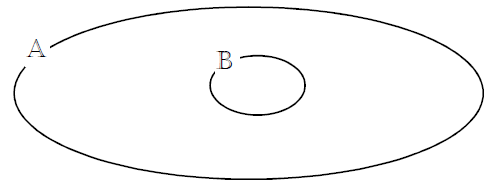
\includegraphics[scale=0.8]{images/teilmenge.png}
        \end{figure}
        Es ist einfach zu erkennen, dass die Menge $B$ vollständig von der grösseren Menge $A$ umschlossen wird und somit alle Elemente von $B$ auch in $A$ enthalten sind.
    \end{beispiel}
    \begin{definition}[leere Menge]
        Eine Menge, die keine Elemente enthält, heisst \textbf{leere Menge} und wird mit $\emptyset$ bezeichnet.
    \end{definition}
    \begin{aufgabe}
        Beschreiben $\emptyset$ und $\{0\}$ dieselbe Menge? Begründe.\vspace{5pt}\newline\karos{3.5}
    \end{aufgabe}
    \begin{satz}
        Die leere Menge ist eine Teilmenge jeder Menge.
    \end{satz}
\subsection{Mengenoperationen}
    Ähnlich wie das Plus, Minus, etc. gibt es für Mengen auch Operationen, mit denen die neue Mengen beschrieben werden können. In diesem Abschnitt werden die drei verschiedenen Mengenoperationen eingeführt. Dazu betrachten wir die beiden Mengen: \[C=\{1,2,3\}\quad\text{ und }\quad D=\{3,4,5\}.\]
    \begin{enumerate}[label=\ ]
            \item\begin{minipage}{0.6\linewidth}
                \textbf{Durchschnitt:} $C\cap D=\gap{5}$\newline
                Die Mengenoperation \glqq Durchschnitt\grqq\:ist eine kommutative Operation. Das heisst: \[C\cap D=D\cap C\]
            \end{minipage}
            \hfill
            \begin{minipage}{0.37\linewidth}
                \centering
                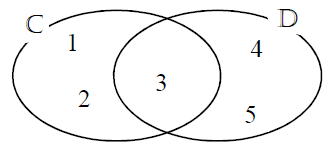
\includegraphics[scale=0.7]{images/operationen.png}
            \end{minipage}\vspace{18pt}
            \item\begin{minipage}{0.6\linewidth}
                \textbf{Vereinigung:} $C\cup D=\gap{5}$\newline
                Die Mengenoperation \glqq Vereinigung\grqq\:ist ebenfalls eine kommutative Operation. Das heisst: \[C\cup D=D\cup C\]
            \end{minipage}
            \hfill
            \begin{minipage}{0.37\linewidth}
                \centering
                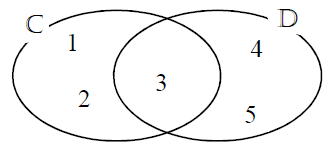
\includegraphics[scale=0.7]{images/operationen.png}
            \end{minipage}\vspace{18pt}
            \item\begin{minipage}{0.6\linewidth}
                \textbf{Differenzmenge:} $C\backslash D=\gap{2}$\newline
                Die Mengenoperation \glqq Differenzmenge\grqq\: ist \textbf{nicht} kommutativ.\[D\backslash C=\gap{3}\neq D\backslash C\]
            \end{minipage}
            \hfill
            \begin{minipage}{0.37\linewidth}
                \centering
                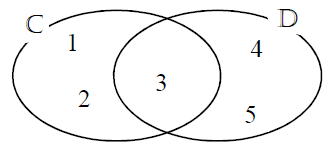
\includegraphics[scale=0.7]{images/operationen.png}
            \end{minipage}
    \end{enumerate}
    \begin{aufgabe}
        Löse die Aufgaben $1-4$ in der Aufgabensammlung.
    \end{aufgabe}


\newpage
\section{Die natürlichen Zahlen}
    \begin{aufgabe}
        \begin{enumerate}
            \item Sabrina wirft drei handelsübliche Spielwürfel gleichzeitig und notiert sich die Summe der drei Augenzahlen. Wie viele und welche Ergebnisse kann sie erhalten?
        \end{enumerate}\karos{3.5}
        \begin{enumerate}\setcounter{enumi}{1}
            \item In einem Teich lebt eine verblüffende Wasserlilienart. Sie wächst nämlich so schnell, dass die Teichfläche, die sie überdeckt, jeden Tag verdoppelt wird. Angenommen die Lilie benötigt $30$ Tage, um den Teich vollständig zu überdecken. Wie viele Tage benötigt sie, um einen viertel des Teichs zu überdecken?
        \end{enumerate}\karos{3.5}
    \end{aufgabe}
    Wir stellen in diesen Aufgaben fest, dass die Zahlen, die darin verwendet werden meistens mit einem Objekt zusammenhängen. Sie sind also sozusagen eine Abstraktion des Zählens. Diese Abstraktion benötigte aber eine Einigung auf ein gemeinsames Zahlensystems. Unser heute gebräuchliches $10-$er System ist euch bereits ausführlich bekannt und wir sind in der Lage mit diesen Zahlen problemlos zu rechnen. Nichts desto trotz benötigen wir für die weiteren Kapitel die exakte Definition dieser Abstraktion.
    \begin{definition}
        Die Menge der natürlichen Zahlen ist die Menge \[\N=\{1,2,3,4,\ldots\}\]
        Die Zahl $0$ spielt beim Zählen eine ganz spezielle Rolle, deshalb kennzeichnen wir klar, falls die $0$ dazu genommen wird. \[\N_0=\{0,1,2,3,4,\ldots\}\]
    \end{definition}
    Wir beherrschen das Rechnen mit natürlichen Zahlen schon gut. Wir wiederholen in diesem Abschnitt Begriffe wie Teiler, Primzahl, $\ggT$ und $\kgV$.
    \begin{definition}
	   Sei $n\in\N$ eine natürliche Zahl. Wir sagen $a\in\N$ ist ein \textbf{Teiler} von $n$, wenn es eine Zahl $b\in\N$ gibt so, dass $a\*b=n$.
    \end{definition}
    \begin{notation}
        Man sagt oft auch \glqq$a$ teilt $n$\grqq\: und schreibt dafür $\mathbf{a|n}$.
    \end{notation}
    \begin{beispiel}
    	Die Teilermenge einer Zahl ist die Menge all ihrer Teiler.
    	\begin{itemize}
    		\item Die Teilermenge von 12 ist: \[T_{12} = \{1, 2, 3, 4, 6, 12\}\]
    		\item Die Teilermenge von 136 ist: \[T_{136} = \{1, 2, 4, 8, 17, 34, 68, 136 \}\]
    		Offensichtlich sind 1 und 136 Teiler. Um alle Teiler zu finden, kann man die Zahlen 2, 3, 4, 5, \ldots testen, ob sie Teiler von 136 sind. Ist einer dieser Kandidaten ein Teiler, dann hat man sofort einen zweiten Teiler gefunden: Findet man beispielweise, dass 8 ein Teiler von 136 ist, dann gilt $136 = 8\*17$ und somit ist auch 17 ein Teiler von 136.
    	\end{itemize}
    \end{beispiel}
    \begin{aufgabe}
        \begin{enumerate}
            \item Benutze die Definition, um in eigenen Worten zu erklären, wieso die folgenden Aussagen wahr sind.
            \begin{enumerate}[label=\alph*)]
                \item Die Zahl $1$ ist Teiler jeder natürlichen Zahl.
                \item Jede natürliche Zahl ungleich $0$ ist ein Teiler von $0$.
                \item Jede natürliche Zahl ist ein Teiler von sich selbst.
            \end{enumerate}
            \item Hier siehst du eine Auflistung von verschiedenen Zahlen: $17,6,24,1,18,5,90$. Notiere alle möglichen Teilerbeziehungen aus zwei Zahlen dieser Liste in der Form $m|n$.
        \end{enumerate}
    \end{aufgabe}
\subsection{Primzahlen}
    Eine ungemein wichtige Klasse von Zahlen sind die sogenannten Primzahlen. Dies hat mehrere Gründe, angefangen bei ihrer immer noch nicht restlos geklärten Frage zur Regelmässigkeit. Es ist mittlerweile bewiesen, dass es unendlich viele Primzahlen gibt, aber auch diese Aussage wurde sehr lange kontroverse diskutiert. Wir starten hier aber bei den Grundlagen und definieren zuerst den Begriff der Primzahl.
    \begin{definition}
        Eine natürliche Zahl $p>1$ heisst \textbf{prim} oder \textbf{Primzahl}, falls sie genau zwei Teiler, nämlich $1$ und sich selbst, hat.
    \end{definition}
    Die Primzahlen werden häufig als die Grundbausteine der natürlichen Zahlen betrachtet. Dabei wird auch klar, warum die Zahl $1$ keine Primzahl sein darf. Dazu betrachten wir die Primfaktorzerlegung.
    \begin{satz}[Fundamentalsatz der Arithmetik]
        Jede natürliche Zahl $n\in\N$ kann \emph{eindeutig} als Produkt von Primzahlen geschrieben werden.
        \[n=p_1^{r_1}\*p_2^{r_2}\*\ldots\*p_s^{r_s}\]
        Dabei sind $p_1,p_2,\ldots,p_s$ eine bestimmte Anzahl an Primzahlen und $r_1,r_2,\ldots,r_s\in\N$ die dazugehörigen Exponenten.\\
        Diese Zerlegung wird \textbf{Primfaktorzerlegung} genannt.
    \end{satz}
    \begin{beispiel}
        Wir suchen die Primfaktorzerlegung von $504$. Dazu stellen wir und schrittweise die Frage, ob $504$ durch eine Primzahl geteilt werden kann. Dabei starten wir mit der kleinsten Primzahl und erhöhen diese schrittweise.
        \begin{enumerate}
            \item Ist $504$ durch $2$ teilbar?
            \item Ist \gap{2} durch \gap{2} teilbar?
        \end{enumerate}
    \end{beispiel}\karos{4.5}
    Insgesamt scheint der Satz offensichtlich zu sein. Dennoch ist der Beweis, dass die Zerlegung eindeutig ist, sehr anspruchsvoll. Aus diesem Grund verzichten wir hier auf einen ausführlichen Beweis. Die Eindeutigkeit ist aber einer der Gründe, wieso die Zahl $1$ keine Primzahl ist. Denn ansonsten könnten mehrere Primfaktorzerlegungen für die gleiche Zahl gefunden werden. \[21=3\*7=1\*3\*7=1^2\*3\*7=1^3\*3\*7=\ldots\]
    Bevor wir in die ersten Aufgaben starten, sind hier noch einige Teilbarkeitstest der kleineren Primzahlen.
    \begin{satz}[Teilbarkeitstests]
        Es gelten folgende Teilbarkeitstests:
        \begin{enumerate}
            \item Die Zahl $n$ ist durch $2$ teilbar $\Leftrightarrow$ Die Zahl $n$ ist gerade.
            \item Die Zahl $n$ ist durch $3$ teilbar $\Leftrightarrow$ Die Quersumme von $n$ ist durch $3$ teilbar.
            \item Die Zahl $n$ ist durch $5$ teilbar $\Leftrightarrow$ Die letzte Ziffer von $n$ ist eine $0$ oder $5$
        \end{enumerate}
    \end{satz}
    Es gibt selbstverständlich auch Teilbarkeitsregeln für $7, 11$ und $13$. Jedoch sind diese Regeln nicht mehr so einfach formulierbar wie die obigen. Falls du diese dennoch nachlesen willst, folge diesem \href{https://www.matheretter.de/wiki}{Link} und suche in der Auflistung nach \glqq Teilbarkeit und Teilbarkeitsregeln\grqq.
    \begin{aufgabe}
        Berechne für die folgenden Zahlen ihre Primfaktorzerlegung.
        \begin{enumerate}[label=\alph*)]
            \item $34=$
            \item $1188=$
            \item $437=$
            \item $8100=$
            \item $36=$
            \item $54254055625=$
        \end{enumerate}
    \end{aufgabe}

\subsection{Grösster gemeinsamer Teiler und kleinstes gemeinsames Vielfach}
    Die Primfaktorzerlegung hilft uns vor allem bei der Suche nach dem grössten gemeinsamen Teiler ($\ggT$) oder dem kleinsten gemeinsamen Vielfach ($\kgV$).
    \begin{definition}
        Der grösste gemeinsame Teiler $\ggT$ ist die größte natürliche Zahl, durch die sich zwei ganze Zahlen ohne Rest teilen lassen.\newline
        Das kleinste gemeinsame Vielfach $\kgV$ ist die kleinste natürliche Zahl, die ein Vielfaches beider ganzen Zahlen ist.
    \end{definition}
    Lasst uns dazu direkt ein Beispiel betrachten und diskutieren, wie diese nun gefunden werden.
    \begin{beispiel}
        Betrachten wir die beiden Zahlen $6468$ und $840$. Zuerst bilden wir die beiden Primfaktorzerlegungen.
        \begin{align*}
            6468&=\hspace{11cm}\\
            840&=
        \end{align*}
        Um den $\ggT(6468,840)$ zu berechnen, müssen wir diejenigen Primfaktoren herauspicken, die in beiden Zerlegungen vorkommen, und dann zu jedem dieser Primfaktoren den kleineren der beiden Exponenten wählen.
        \begin{align*}
            6468&=\hspace{11cm}\\
            840&=
        \end{align*}
        Um den $\kgV(6468,840)$ zu berechnen, müssen wir hingegen diejenigen Primfaktoren suchen, die in mindestens einer der beiden Zerlegungen vorkommen, und zu jefem dieser Primfaktoren den grösseren der beiden Exponenten wählen.
        \begin{align*}
            6468&=\hspace{11cm}\\
            840&=
        \end{align*}
    \end{beispiel}
    \begin{aufgabe}
        Berechne das $\kgV$ und den $\ggT$ der beiden gegebene Zahlen.
        \begin{enumcols}[3]
            \item $308,210$
            \item $153,255$
            \item $468,572$
            \item $208,351$
            \item $294,315$
            \item $1144,748$
        \end{enumcols}
    \end{aufgabe}
    Leider ist das Herstellen der Primfaktorzerlegung gerade bei sehr grossen Zahlen extrem aufwendig, weil es bis heute keinen effizienten Algorithmus gibt. Je nach grösse der Zahl kann eine solche vom Computer durchgeführte Berechnung der Zerlegung Stunden, Tage, Jahre oder sogar Milliarden von Jahren dauern. Aus diesem Grund basieren viele moderne Verschlüsselungssysteme gerade darauf, da diese Zerlegung nicht in nützlicher Frist berechnet werden kann. So wird garantiert, dass kein nicht autorisierter Nutzer auf bestimmte Daten zugreifen kann.\newpage


\section{Die ganzen Zahlen}
    Um gewisse Gleichungen zu lösen, reichen die natürlichen Zahlen nicht mehr aus:
    \[5 + x = 2\]
    Um solche und ähnliche Probleme zu lösen, führt man negative Zahlen ein, welche zusammen mit den natürlichen Zahlen und der $0$ eine neue Zahlenmenge bilden:
    \begin{definition}[Ganze Zahlen]
        Die Menge der ganzen Zahlen  ist die Menge
        \[\Z = \{ \ldots, -2, -1, 0, 1, 2, 3, 4, \ldots\}\]
        Eine ganze Zahl $n$ ist definiert durch ihr \emph{Vorzeichen} ($ + $ oder $ - $) und ihren \emph{Betrag} $\abs{n}$. Der Betrag ist dabei folgendermassen definiert:
        \[\abs{n} = \begin{cases} n &\text{ falls } n>0 \\ -n &\text{ falls } n<0 \end{cases}\]
    \end{definition}\vspace{5pt}
    \begin{minipage}{0.47\linewidth}
        Wir sehen, dass die natürlichen Zahlen in den ganzen Zahlen enthalten sind. Man sagt, die Menge der natürlichen Zahlen $\N$ ist eine Teilmenge der ganzen Zahlen $\Z$.
    \end{minipage}
    \hfill
    \begin{minipage}{0.47\linewidth}
        %Venn Diagramm mit \Z und \N
    \end{minipage}
    \begin{beispiel}\
    	\begin{itemize}
    		\item Die Zahl $-3$ hat negatives Vorzeichen ($-$) und den Betrag $\abs{-3} =3$.
    		\item Die Zahl $12$ hat positives Vorzeichen ($+$) und den Betrag $\abs{12} = 12$.
    		\item Die Zahl $0$ hat kein Vorzeichen und den Betrag $\abs{0} = 0$.
    	\end{itemize}
    \end{beispiel}
    Im Zusammenhang mit dieser neuen Zahlenmenge $\Z$ gibt es einen weiteren zentralen Begriff zu definieren.
    \begin{definition}[Gegenzahl]
        Die \textbf{Gegenzahl} einer Zahl $a\in\Z$ ist diejenige Zahl $x\in\Z$, welche denselben Betrag aber das umgekehrte Vorzeichen wie $a$ besitzt. Dabei gilt immer \[a+x=0\]
        Ist $x$ die Gegenzahl von $a$, so schreiben wir $x=-a$
    \end{definition}
    Um uns ans Umgehen mit Beträgen zu gewöhnen, lösen wir noch ein Beispiel dazu. Grundsätzlich kann man Betragsstriche als Klammern sehen, welche \glqq das Vorzeichen entfernen\grqq.
    \begin{beispiel}
    	Wir vereinfachen Terme mit Betragsstrichen:
    	\[\abs{8\*(2 - 5)} + 3\*\abs{2 - \abs{14 + 1} + \abs{-3}\*\abs{4}} - \abs{3 - 7}= \]\karos{2.5}
    	\[-\abs{\frac{3}{4} - \frac{21}{10}} + \abs{\frac{3}{2}\abs{\left(\frac{1}{4} + \frac{1}{5}\right)}} - \abs{\frac{12}{5}\*\left(-\frac{15}{8}\right)}=\]\karos{3.5}
    \end{beispiel}
    \begin{aufgabe}
        Löse die beiden Aufgaben $16$ und $17$ in der Aufgabensammlung.
    \end{aufgabe}\newpage


\section{Die rationalen Zahlen}
    Die ganzen Zahlen sind unter Addition (und Subtraktion) abgeschlossen. D.h. jede Summe (und jede Differenz) zweier ganzer Zahlen ist wieder eine ganze Zahl. Falls ihr später mal Mathematik studieren möchtet, werdet ihr ein solches Objekt als \glqq Gruppe\grqq\: kennenlernen. \newline
    Bezüglich der Multiplikation sind die ganzen Zahlen aber nicht abgeschlossen, denn beispielsweise hat die Gleichung
    \[5\*x = 2\]
    keine Lösung in $\Z$. Wir müssen also unsere Zahlenmenge noch weiter vergrössern.
    \begin{definition}[Rationale Zahlen]
    	Die Menge der \emph{rationalen Zahlen} ist die Zahlenmenge
    	\[\Q = \left\{\frac{z}{n} \Big| z, n\in\Z, n\neq 0 \right\}\]
    	Die Zahl $z$ heisst \emph{Zähler}, die Zahl $n$ heisst \emph{Nenner}.
    \end{definition}
    Statt von rationalen Zahlen spricht man oft auch von \glqq Brüchen\grqq\: oder \glqq Bruchzahlen\grqq. Der Begriff \glqq rational\grqq\: leitet sich vom lateinischen Wort \glqq ratio\grqq\: ab, was \glqq Verhältnis\grqq\: bedeutet. Jede ganze (und somit auch jede natürliche Zahl) kann als Bruchzahl geschrieben werden, z.B. $-5=\frac{-5}{1}$. Dementsprechend sind die ganzen Zahlen eine Teilmenge der rationalen Zahlen: $\N\subset\Z\subset\Q$.\vspace{3cm}\newline
    Eine rationale Zahl kann auf verschiedene Arten dargestellt werden: als verschiedene Bruchzahlen oder als Dezimalzahl.\vspace{2cm}\newline
    Damit wir diese verschiedenen Darstellungen auch vom einen ins andere umformen können, betrachten wir die folgende Definition.
    \begin{definition}
        Eine Dezimalbruchentwicklung einer Zahl ist von der Form $ n.a_{1}a_{2}a_{3}a_{4}\ldots $ wobei $n\in\Z$ eine ganze Zahl ist und $a_{0}, a_{1}, a_{2}, \ldots $ Ziffern aus $\{0,1,\ldots8,9\} $ sind.
        \begin{itemize}
        	\item Eine Dezimalbruchentwicklung heisst \textbf{endlich}, falls ab einer Stelle alle $ a_{i}=0 $ sind.
        	\item Eine Dezimalbruchentwicklung heisst \textbf{periodisch}, falls sie unendlich ist und sich ab einer Stelle die Ziffernfolge wiederholt. Die Länge der Ziffernfolge bestimmt die Länge der Periode.
        \end{itemize}
    \end{definition}
    \begin{beispiel}\
        \begin{itemize}
            \item endlich: $\frac{3}{8}=0.375$ d.h. $n=\gap{1}$ und $a_1=\gap{1},a_2=\gap{1},a_3=\gap{1},a_4=\gap{1},\ldots$
            \item periodisch: $\frac{81}{11}=7.363636\ldots=7.\overline{36}$ d.h. $n=\gap{1}$ und $a_1=\gap{1},a_2=\gap{1},$\newline$a_3=\gap{1},a_4=\gap{1},\ldots$. Man sagt also, $\frac{81}{11}$ hat die Periode $36$ und somit Länge $2$.
        \end{itemize}
    \end{beispiel}
    \begin{aufgabe}
        Wandle die folgenden Brüche in eine Dezimalzahl um. Welche sind endlich und welche sind periodisch?
        \begin{enumcols}[3]
            \item $\displaystyle\frac{8}{5}$
            \item $\displaystyle\frac{1}{8}$
            \item $\displaystyle\frac{15}{13}$
            \item $\displaystyle\frac{7}{20}$
            \item $\displaystyle\frac{11}{6}$
            \item $\displaystyle\frac{9}{7}$
        \end{enumcols}
    \end{aufgabe}
    Umgekehrt kann man auch jede endliche oder periodische Dezimalbruchentwicklung in einen Bruch umwandeln. Dazu betrachten wir das nächste Beispiel.
    \begin{beispiel}
    	Gewisse Dezimalbrüche erkennt man \glqq aus Erfahrung\grqq:
    		\[3.25 = \frac{13}{4} \qquad 0.625 = \frac{5}{8} \qquad 0.7 = \frac{7}{10}\]
    		Ist der Bruch nicht so offensichtlich erkennbar, so kann man ihn immer als einen Bruch mit einer 10er Potenz als Nenner schreiben. Anschliessend wird der Bruch so weit wie möglich gekürzt.
    		\begin{align*}
    			0.84 &= \frac{84}{100} = \frac{21}{25} \\
    			2.34 &= \frac{234}{100} = \frac{117}{50} \\
    			1.0012 &= \frac{10012}{10000} = \frac{2503}{2500}
    		\end{align*}
    \end{beispiel}
    Viel interessanter sind aber periodische Dezimalbrüche. Studiere dazu folgendes Beispiel
    \begin{beispiel}
        Erkläre in eigenen Worten, was in diesem Beispiel gemacht wird.\newline
        Wir suchen die Bruchzahl $x$, welche zur periodischen Dezimalzahl $0.\overline{7}$ gehört. Dazu gehen wir wie folgt vor:
        \begin{table}[H]
            \centering
            \begin{tabular}{p{1.5cm} p{3cm} c}
                I: & $\:\:x=0.7777777\ldots$ & $\vert\*10$\\
                II: & $10x=7.777777\ldots$ & \\\hline
                II$\:-\:$I: & $10x-x=7$ & \\
                & \hspace{24pt}$9x=7$ & $\vert\div 9$\\
                & \hspace{28pt}$\displaystyle x=\frac{7}{9}$ &
            \end{tabular}
        \end{table}
    \end{beispiel}
    \begin{aufgabe}
        Löse die Aufgaben $5-9$ aus der Aufgabensammlung.
    \end{aufgabe}\newpage


\section{Die reelen Zahlen}
    Die reelen Zahlen bilden unseren Abschluss unserer Zahlenräume. Um aber besser zu verstehen, welche Zahlen hier noch dazugekommen sind, bearbeite folgende Aufgabe.
    \begin{aufgabe}
        Wir haben gelernt, dass die Dezimalbruchentwicklung einer rationalen Zahl stets entweder endlich oder periodisch ist. Notiere hier Beispiele von Zahlen die diese beiden Eigenschaften \textbf{nicht} erfüllen.\vspace{5pt}\newline\karos{3.5}
        Wie viele solcher Zahlen gibt es denn?\vspace{5pt}\newline\karos{1.5}
    \end{aufgabe}
    \begin{definition}[Irrationale Zahlen]
        Dezimalbrüche, die unendlich und nicht-periodisch sind, nennen wir irrationale Zahlen. Man schreibt dafür $\I$.
    \end{definition}
    Als Konsequenz können wir nun den grössten und für uns interessantesten Zahlenraum definieren.
    \begin{definition}[Reelle Zahlen]
        Die Menge der \textbf{reellen Zahlen} ist die Vereinigung der Menge der rationalen Zahlen $\Q$ und der Menge der irrationalen Zahlen $\I$. \[\R=\Q\cup\I\]
        Einfach gesagt, zu den reellen Zahlen gehören alle möglichen Dezimalbrüche. \[\R=\left\{n.a_1a_2a_3\ldots\vert n\in\Z,a_1,a_2,a_3,\ldots\in\{0,1,\ldots9\}\right\}\]
    \end{definition}\vspace{5pt}
    \begin{minipage}{0.47\linewidth}
        Die natürlichen, ganzen, rationalen und irrationalen Zahlen sind alle auch reelle Zahlen. Somit sind die entsprechenden Zahlenmengen Teilmengen von $\R$.\newline
        Es gilt $\N\subset\Z\subset\Q\subset\R$.
    \end{minipage}
    \hfill
    \begin{minipage}{0.47\linewidth}
        %Venn Diagramm mit \R bis \N
    \end{minipage}\vspace{24pt}\newline
    Diese vier Zahlenmengen bilden die Grundlage aller unserer weiteren Konzepten. In der Primarschule habt ihr bestimmt die Zahlengerade benutzt, um Zahlen darin einzuzeichnen. Zeichnen wir doch unsere Zahlenmengen ebenfalls hier ein.
    \begin{figure}[H]
        \centering
        \begin{tikzpicture}[line cap=round,line join=round,>=triangle 45,x=1.0cm,y=1cm]
            \draw[->](-5,0) --(8,0);
            \foreach \x in {-4.,-3.,-2.,-1.,0.,1.,2.,3.,4.,5.,6.,7.}
            \draw[shift={(\x,0)},color=black] (0pt,2pt) -- (0pt,-2pt) ;%node[below] {\footnotesize $\x$};
            \draw[color=black] (8,0) node[right] {$\R$};
        \end{tikzpicture}
    \end{figure}\vspace{2cm}

\subsection{Rechengesetze}
    Da wir nun unseren Zahlengerade gefüllt haben, sollten wir uns noch kurz über die geltenden Rechengesetze unterhalten. Dabei wird davon ausgegangen, dass  diese Gesetze bereits bekannt sind und es ist somit nur eine Repetition.
    \begin{satz}[grundlegende Rechengesetze]
        Sind $a,b$ und $c$ beliebige reelle Zahlen, so gilt:
        \begin{table}[H]
            \begin{tabular}{p{8cm} c}
                Kommitativgesetz der Addition: & $a+b=b+a$ \\
                Kommutativgesetz der Multiplikation: & $a\*b=b\*a$\\
                Assoziativgesetz der Addition: & $(a+b)+c=a+(b+c)$ \\
                Assoziativgesetz der Multiplikation: & $(a\*b)\*c=a\*(b\*c)$ \\
                Dristributivgesetze: & $a\*(b\pm c)=a\*b\pm a\*c$ \\
                & $(a\pm b)\*c=a\*c\pm b\*c$
            \end{tabular}
        \end{table}
    \end{satz}

\subsection{Der Betrag einer reellen Zahl}
    Weiter können wir den Betrag einer Zahl, wie wir ihn im Abschnitt zu den ganzen Zahlen kennen gelernt haben, auf die Menge der reellen Zahlen erweitern.
    \begin{definition}
        Sei $x\in\R$ eine beliebige reelle Zahl, so ist der Betrag von $x$ definiert als \[\abs{x} = \begin{cases} x &\text{ falls } x\geq0 \\ -x &\text{ falls } x<0. \end{cases}\]
    \end{definition}
    Wir sehen es gibt überhaupt keinen Unterschied, ausser dass die Zahl nun eine reelle Zahl sein darf.

\subsection{Approximation}
    Da reelle Zahlen teils nicht exakt angegeben werden können, sollten wir ein Symbol einführen, das deutlich macht, dass wir eine Zahl nur näherungsweise angegeben. Zum Beispiel können wir die Nachkommastellen von $\sqrt{2}$ niemals alle aufschreiben, da sie eine unendliche und nicht periodische Dezimalbruchentwicklung besitzt. Wenn wir also mit $n$ die Wurzel von $2$ meinen, dann schreiben wir entweder $n=\sqrt{2}$ für die abstrakte Notation oder $n\approx 1.414$ für den gerundeten Wert.
    \begin{notation}
        Falls wir eine Zahl nur näherungsweise angeben, z.B. in Form eines gerundeten Dezimalbruches, so verwenden wir das $\approx$ Symbol.
    \end{notation}

\subsection{Intervalle}
    Oftmals wollen wir von der Zahlengerade nur einen Ausschnitt davon angeben. Dieser Ausschnitt startet bei einer kleinsten Zahl und und endet mit einer grössten Zahl. Einen solchen Ausschnitt wird in der Mathematik \glqq Intervall\grqq\: genannt. Dabei werden vier verschiedene Intervalle unterschieden:
    \begin{definition}[Intervall]
        Intervalle sind Teilmengen der reellen Zahlen, wobei sie alle Zahlen umfassen, die zwischen den beiden Grenzen liegen. Dabei wird noch unterschieden, ob die Grenzen dazugehören oder nicht:
        \begin{enumerate}[label=\alph*)]
            \item \textbf{abgeschlossenes} Intervall\newline
            \begin{minipage}{0.60\linewidth}
                \[[a,b]=\{x\in\R\vert a\leq x\leq b\}\]
                Die Grenzen gehören hier dazu!
            \end{minipage}
            \hfill
            \begin{minipage}{0.37\linewidth}
                \centering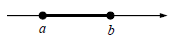
\includegraphics[scale=1]{images/geschlossen.png}
            \end{minipage}
            \item \textbf{offenes} Intervall\newline
            \begin{minipage}{0.60\linewidth}
                \[]a,b[=\{x\in\R\vert a<x<b\}\]
                Die Grenzen gehören hier \textbf{nicht} dazu!
            \end{minipage}
            \hfill
            \begin{minipage}{0.37\linewidth}
                \centering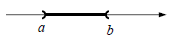
\includegraphics[scale=1]{images/offen.png}
            \end{minipage}
            \item \textbf{halboffenes} Intervall (nach links)\newline
            \begin{minipage}{0.60\linewidth}
                \[]a,b]=\{x\in\R\vert a<x\geq b\}\]
                Nur die rechte Grenzen gehört dazu!
            \end{minipage}
            \hfill
            \begin{minipage}{0.37\linewidth}
                \centering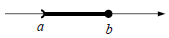
\includegraphics[scale=1]{images/halboffenlinks.png}
            \end{minipage}
            \item \textbf{halboffenes} Intervall (nach rechts)\newline
            \begin{minipage}{0.60\linewidth}
                \[[a,b[=\{x\in\R\vert a\geq x<b\}\]
                Nur die linke Grenzen gehört dazu!
            \end{minipage}
            \hfill
            \begin{minipage}{0.37\linewidth}
                \centering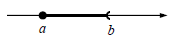
\includegraphics[scale=1]{images/halboffenrechts.png}
            \end{minipage}
        \end{enumerate}
    \end{definition}
    Das Zeichen $\infty$ heisst \textbf{unendlich} und beschreibt den Ort auf der Zahlengerade, der unendlich weit rechts auf ihr liegt. Weil $\infty$ keine scharfe Grenze darstellt, muss dort immer eine offene Intervallgrenze verwendet werden. Hier sind einige Beispiele:
    \begin{enumcols}[2]
        \item $[-3,\infty[ = \{x\in\R\vert x\geq -3\}$
        \item $]7,\infty[=\{x\in\R\vert x>7\}$
        \item $]-\infty,2[=\{x\in\R\vert x<2\}$
        \item $]-\infty,-5]=\{x\in\R\vert x\leq -5\}$
    \end{enumcols}
    \begin{aufgabe}
        Stelle die folgenden Teilmengen als Intervalle dar.
        \begin{enumcols}[2]
            \item $\{x\in\R\vert\:2.2<x\leq 12.7\}=$
            \item $\{x\in\R\vert\:2.2\geq x>-3.7\}=$
            \item $\{x\in\R\vert\:x>4\}=$
            \item $\{x\in\R\vert\:4>x\}=$
            \item $\R\backslash\{0\}=$
            \item $\R^+\backslash\{5\}=$
            \item $\R_0^+\backslash\{1,7\}=$
            \item $\R\backslash[-1,3]=$
            \item $\R\backslash]2,5[=$
            \item $\R^-\backslash\{1,3,7\}$
        \end{enumcols}
    \end{aufgabe}


\newpage
\subsection*{History}
\begin{table}[H]
    \centering
    \begin{tabular}{|p{13mm}|p{20mm}|p{30mm}|p{70mm}|}\hline
        %\multicolumn{4}{|l|}{History}\\\hline
        Version & Datum & Person & Bemerkung \\\hline
        $0.1$ & 02.08.2024 & Jonas Guler & Kapitel erstellt \\\hline
         & ToDo & Jonas Guler & \\\hline
    \end{tabular}
\end{table}

\end{document}